%% Преамбула TeX-файла

% 1. Стиль и язык
\documentclass{G7-32} % Стиль (по умолчанию размер шрифта 14pt)

% Остальные стандартные настройки убраны в preamble.inc.tex.
\sloppy

% Настройки стиля ГОСТ 7-32
% Для начала определяем, хотим мы или нет, чтобы рисунки и таблицы нумеровались в пределах раздела, или нам нужна сквозная нумерация.
\EqInChapter % формулы будут нумероваться в пределах раздела
\TableInChapter % таблицы будут нумероваться в пределах раздела
\PicInChapter % рисунки будут нумероваться в пределах раздела

% Добавляем гипертекстовое оглав\usepackage{iftex}ление в PDF
\usepackage[
bookmarks=true, colorlinks=true, unicode=true,
urlcolor=black,linkcolor=black, anchorcolor=black,
citecolor=black, menucolor=black, filecolor=black,
]{hyperref}

\AfterHyperrefFix

\usepackage{microtype}% полезный пакет для микротипографии, увы под xelatex мало чего умеет, но под pdflatex хорошо улучшает читаемость

% Тире могут быть невидимы в Adobe Reader
\ifInvisibleDashes
\MakeDashesBold
\fi

\usepackage{graphicx}   % Пакет для включения рисунков

% С такими оно полями оно работает по-умолчанию:
% \RequirePackage[left=20mm,right=10mm,top=20mm,bottom=20mm,headsep=0pt,includefoot]{geometry}
% Если вас тошнит от поля в 10мм --- увеличивайте до 20-ти, ну и про переплёт не забывайте:
\geometry{right=20mm}
\geometry{left=30mm}
\geometry{bottom=20mm}
\geometry{ignorefoot}% считать от нижней границы текста


% Пакет Tikz
\usepackage{tikz}
\usetikzlibrary{arrows,positioning,shadows}

% Произвольная нумерация списков.
\usepackage{enumerate}

% ячейки в несколько строчек
\usepackage{multirow}

% itemize внутри tabular
\usepackage{paralist,array}

%\setlength{\parskip}{1ex plus0.5ex minus0.5ex} % разрыв между абзацами
\setlength{\parskip}{1ex} % разрыв между абзацами
\usepackage{blindtext}

% Центрирование подписей к плавающим окружениям
%\usepackage[justification=centering]{caption}

\usepackage{newfloat}
\DeclareFloatingEnvironment[
placement={!ht},
name=Equation
]{eqndescNoIndent}
\edef\fixEqndesc{\noexpand\setlength{\noexpand\parindent}{\the\parindent}\noexpand\setlength{\noexpand\parskip}{\the\parskip}}
\newenvironment{eqndesc}[1][!ht]{%
    \begin{eqndescNoIndent}[#1]%
\fixEqndesc%
}
{\end{eqndescNoIndent}}

\usepackage{svg}
\usepackage{minted}
\usepackage{pdfpages}




% Настройки листингов.
\ifPDFTeX
% 8 Листинги

\usepackage{listings}

% Значения по умолчанию
\lstset{
  basicstyle= \footnotesize,
  breakatwhitespace=true,% разрыв строк только на whitespacce
  breaklines=true,       % переносить длинные строки
%   captionpos=b,          % подписи снизу -- вроде не надо
  inputencoding=koi8-r,
  numbers=left,          % нумерация слева
  numberstyle=\footnotesize,
  showspaces=false,      % показывать пробелы подчеркиваниями -- идиотизм 70-х годов
  showstringspaces=false,
  showtabs=false,        % и табы тоже
  stepnumber=1,
  tabsize=4,              % кому нужны табы по 8 символов?
  frame=single
}

% Стиль для псевдокода: строчки обычно короткие, поэтому размер шрифта побольше
\lstdefinestyle{pseudocode}{
  basicstyle=\small,
  keywordstyle=\color{black}\bfseries\underbar,
  language=Pseudocode,
  numberstyle=\footnotesize,
  commentstyle=\footnotesize\it
}

% Стиль для обычного кода: маленький шрифт
\lstdefinestyle{realcode}{
  basicstyle=\scriptsize,
  numberstyle=\footnotesize
}

% Стиль для коротких кусков обычного кода: средний шрифт
\lstdefinestyle{simplecode}{
  basicstyle=\footnotesize,
  numberstyle=\footnotesize
}

% Стиль для BNF
\lstdefinestyle{grammar}{
  basicstyle=\footnotesize,
  numberstyle=\footnotesize,
  stringstyle=\bfseries\ttfamily,
  language=BNF
}

% Определим свой язык для написания псевдокодов на основе Python
\lstdefinelanguage[]{Pseudocode}[]{Python}{
  morekeywords={each,empty,wait,do},% ключевые слова добавлять сюда
  morecomment=[s]{\{}{\}},% комменты {а-ля Pascal} смотрятся нагляднее
  literate=% а сюда добавлять операторы, которые хотите отображать как мат. символы
    {->}{\ensuremath{$\rightarrow$}~}2%
    {<-}{\ensuremath{$\leftarrow$}~}2%
    {:=}{\ensuremath{$\leftarrow$}~}2%
    {<--}{\ensuremath{$\Longleftarrow$}~}2%
}[keywords,comments]

% Свой язык для задания грамматик в BNF
\lstdefinelanguage[]{BNF}[]{}{
  morekeywords={},
  morecomment=[s]{@}{@},
  morestring=[b]",%
  literate=%
    {->}{\ensuremath{$\rightarrow$}~}2%
    {*}{\ensuremath{$^*$}~}2%
    {+}{\ensuremath{$^+$}~}2%
    {|}{\ensuremath{$|$}~}2%
}[keywords,comments,strings]

% Подписи к листингам на русском языке.
\renewcommand\lstlistingname{Листинг}
\renewcommand\lstlistlistingname{Листинги}

\else
\usepackage{local-minted}
\fi

% Полезные макросы листингов.
% Любимые команды
\newcommand{\Code}[1]{\textbf{#1}}

% Стиль кода
\usepackage{etoolbox,xpatch}

\makeatletter
\AtBeginEnvironment{minted}{\dontdofcolorbox}
\def\dontdofcolorbox{\renewcommand\fcolorbox[4][]{##4}}
\xpatchcmd{\inputminted}{\minted@fvset}{\minted@fvset\dontdofcolorbox}{}{}
\xpatchcmd{\mintinline}{\minted@fvset}{\minted@fvset\dontdofcolorbox}{}{} % see https://tex.stackexchange.com/a/401250/
\makeatother

\usemintedstyle[cs]{bw}
\newcommand{\inputmintedgray}[2]{%
	\begingroup

	\inputminted[fontsize=\footnotesize, breaklines, breakanywhere, breakautoindent=false, baselinestretch=1]{#1}{#2}

	\endgroup
}



\begin{document}

\frontmatter % выключает нумерацию ВСЕГО; здесь начинаются ненумерованные главы: реферат, введение, глоссарий, сокращения и прочее.

\maketitle %создает титульную страницу





%\listoffigures                         % Список рисунков

%\listoftables                          % Список таблиц

%\NormRefs % Нормативные ссылки 
% Команды \breakingbeforechapters и \nonbreakingbeforechapters
% управляют разрывом страницы перед главами.
% По-умолчанию страница разрывается.

% \nobreakingbeforechapters
\breakingbeforechapters



\tableofcontents

\printnomenclature % Автоматический список сокращений


\mainmatter % это включает нумерацию глав и секций в документе ниже

\chapter{Постановка задачи}

\section{Задание 1}

Разработать класс, согласно индивидуальному варианту, содержащий:

\begin{enumerate}
	\item элементы разного уровня доступа (public и private);
	\item не менее четырех свойств; 
	\item не менее трех методов;
	\item перегрузку метода ToString();
	\item статический метод;
	\item константное или поле только для чтения;
	\item не менее трех конструкторов;
	\item перегрузку операции присваивания и одной любой арифметической.
\end{enumerate}

--

Разработать класс, согласно индивидуальному варианту, содержащий:

\begin{itemize}
	\item элементы разного уровня доступа (public и private);
	\item не менее четырех свойств; 
	\item не менее трех методов;
	\item перегрузку метода ToString();
	\item статический метод;
	\item константное или поле только для чтения;
	\item не менее трех конструкторов;
	\item перегрузку операции присваивания и одной любой арифметической.
\end{itemize}

Рекомендуемые поля и методы указаны в варианте. Также необходимо написать программу с меню, позволяющую протестировать
разработанный класс. Обязательные пункты меню:
\begin{itemize}
	\item задание параметров конструируемого объекта;
	\item вывод свойств объекта;
	\item выполнение статического метода;
	\item выполнение методов объекта.
\end{itemize}


\chapter{Реализация}

\section{Файл ProgramFirst}

\inputmintedgray{cs}{code/ProgramFirst.cs}
\chapter{Результаты работы программы}

Внутри программы реализовано меню с выбором нужного задания, это мы можем увидеть на рисунке \ref{fig:tasks}

\begin{figure}
	\centering
	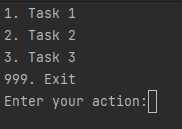
\includegraphics{inc/1}
	\caption{Меню выбора задания}
	\label{fig:tasks}
\end{figure}

\section{Задание 1}

На рисунке \ref{fig:1actions} мы можем видеть меню выбора действия

\begin{figure}
	\centering
	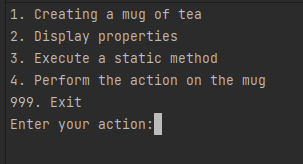
\includegraphics{inc/2}
	\caption{Меню выбора действия}
	\label{fig:1actions}
\end{figure}


\backmatter %% Здесь заканчивается нумерованная часть документа и начинаются ссылки и
           
\Conclusion

Выполняя учебно-практическую работу была разработана программа реализующая работу с классами и интерфейсом.




\end{document}

%%% Local Variables:
%%% mode: latex
%%% TeX-master: t
%%% End:
